% !TeX spellcheck = fr_FR

% TODO: Replace scan images with clean text where possible

\documentclass[a4paper, 10pt]{report}

\usepackage[french]{babel}
\usepackage[T1]{fontenc}

\usepackage{amsmath, amssymb, amsfonts}

\usepackage{hyperref}
\usepackage{geometry}

\usepackage{xcolor}
\usepackage{graphicx}

\usepackage{fancyhdr}
\usepackage{lastpage}

\usepackage{enumitem}

\geometry{
	a4paper,
	left=25mm,
	right=25mm,
	top=35mm,
	bottom=25mm,
	headsep=5mm,
	headheight=20mm,
}

\definecolor{solution}{HTML}{E5E4E2}
\providecommand{\abs}[1]{\lvert#1\rvert}
\providecommand{\norm}[1]{\lVert#1\rVert}
\DeclareMathOperator{\card}{card}

\begin{document}
	
	\renewcommand{\headrule}{%
		\vspace{-4pt}\hrulefill
		\raisebox{-6.8pt}{\ 
\includegraphics[height=5mm]{../../icon.png}}
		\hrulefill
	}	
	\pagestyle{fancy}
	\fancyhf{}
	
	\fancyhead[L]{\small \slshape Automne 2024}
	\fancyhead[C]{\Large \bfseries Analyse I - Série 08}
	\fancyhead[R]{\small Buff Mathias}
	\fancyfoot[L]{
		\small Source files available at:
		\href{https://github.com/MathiasBuff/bsc-math}
		{github.com/MathiasBuff/bsc-math}
	}
	\fancyfoot[R]{
		\small Page \thepage
		\hspace{1pt} /
		\pageref*{LastPage}
	}
	

	\noindent
	\textbf{Exercice 1.} Calculer la dérivée de la fonction
	$f(x) = (x^4 + x^2 - 1)^{41223791150}$.
	
	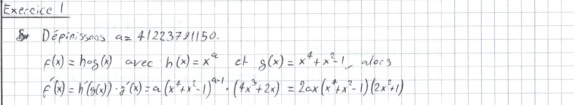
\includegraphics{ex01.jpg}
	
	\vspace{5mm}
	\noindent
	\textbf{Exercice 2.} 
	\begin{enumerate}[label=(\roman*)]
		\item Quelle est l'assertion correspondant à la phrase
		"$f$ tend vers $+\infty$ en $+\infty$" ?
		%
		\item Montrer que si $f$ tend vers $+\infty$ en $+\infty$
		et vérifie $f(x) \neq 0$ pour tout $x \in \mathbb{R}$,\\
		alors $\frac{1}{f}$ tend vers $0$ en $+\infty$.
	\end{enumerate}
	
	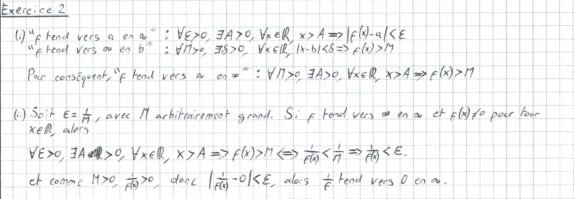
\includegraphics{ex02.jpg}
	
	\vspace{5mm}
	\noindent
	\textbf{Exercice 3.} (Formule de Leibniz).
	Soient $f, g \in C^n(I, \mathbb{R})$. Montrer par récurrence que
	$fg \in C^n(I, \mathbb{R})$ et
	\[(fg)^{(n)} = \sum_{k=0}^{n}\binom{n}{k}f^{(k)}f^{(n-k)}\]
	
	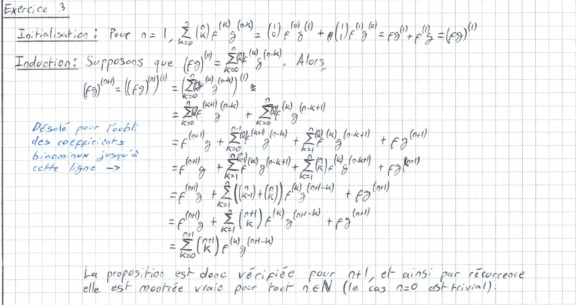
\includegraphics{ex03.jpg}
		
	\newpage

	\fancyhf{}
	\renewcommand{\headrule}
	{\rule{\textwidth}{0pt}}
	\fancyfoot[R]{
		\small Page \thepage
		\hspace{1pt} /
		\pageref*{LastPage}
	}
	
	\noindent
	\textbf{Exercice 4.} Calculer la dérivée $n$-ième des fonctions
	suivantes :
	\begin{enumerate}[label=(\roman*)]
		\item $x \mapsto \dfrac{1}{1 - x}$
		
		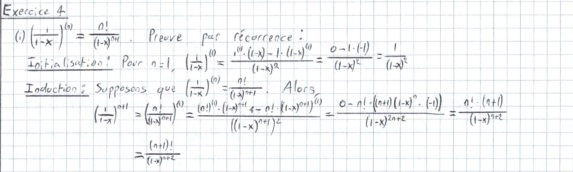
\includegraphics{ex04-p1.jpg}
		
		\item $x \mapsto x^2( 1 + x)^n$
		
		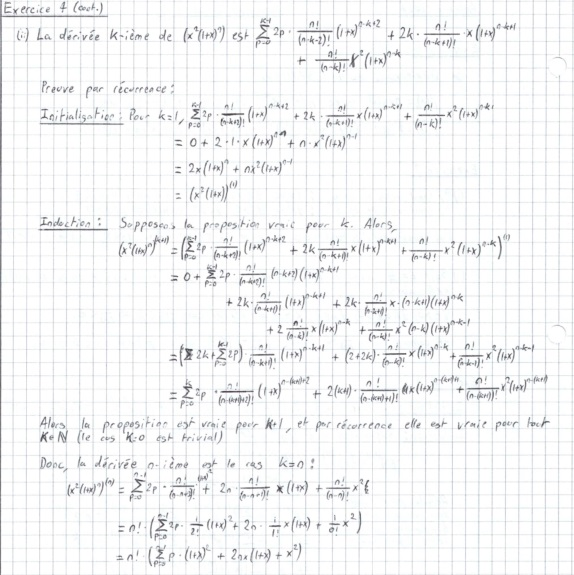
\includegraphics{ex04-p2.jpg}
		
		\item $x \mapsto x^n(1 + x)^n$
		
		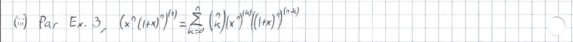
\includegraphics{ex04-p3.jpg}
	\end{enumerate}
	
	\newpage
	
	\noindent
	\textbf{Exercice 5.} (Formulation de Weierstrass de la dérivée).\\
	Montrer que $f: I \to \mathbb{R}$ est continue sur $I$ et dérivable
	en $a$ ssi il existe $\phi: I \to \mathbb{R}$ continue sur $I$
	telle que \[f(x) = f(a) + (x - a) \phi(x), \quad \forall x \in I\]
	
	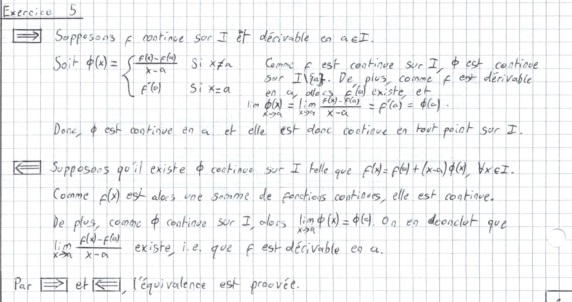
\includegraphics{ex05.jpg}	
		
	\vspace{5mm}
	\noindent
	\textbf{Exercice 6.} Déterminer le domaine de définition puis
	trouver la dérivée en tout point de ce domaine pour la fonction
	$x \mapsto \sqrt{x + \sqrt{1 + x^2}}$.
	
	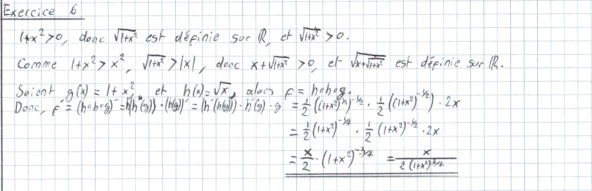
\includegraphics{ex06.jpg}
		
	\vspace{5mm}	
	\noindent
	\textbf{Exercice 7.} Trouver le polynôme de Taylor $T_4f(x;1)$ de
	la fonction $x \mapsto x^{1/3}$. L'utiliser pour calculer
	$(1/2)^{1/3}$, et à l'aide du Théorème de Taylor donner un majorant
	pour l'erreur entre $(1/2)^{1/3}$ et son approximation.
	
	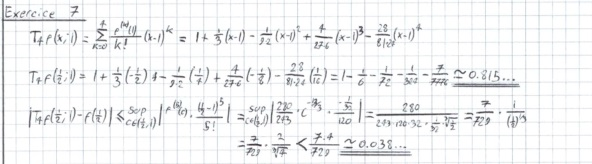
\includegraphics{ex07.jpg}
	
	

	
%	
%	
%	\colorbox{solution}
%	{
%		\begin{minipage}{0.9\textwidth}
%			s
%		\end{minipage}
%	}
%	
%	\colorbox{solution}
%	{
%		\begin{minipage}{0.9\textwidth}
%			\begin{enumerate}[label=(\alph*)]
%				\item a
%			\end{enumerate}
%		\end{minipage}
%	}
	
\end{document}
